\documentclass[UTF8]{ctexart}
\usepackage{amsmath}
\usepackage{graphicx}
\usepackage{float}
\usepackage{subfigure}
\usepackage{xeCJK}
\usepackage{hyperref}
\usepackage{algorithm2e}
\usepackage{amsfonts}
\usepackage{epsfig}
\usepackage{listings}
\usepackage{xcolor}
% 定义可能使用到的颜色

\definecolor{CPPLight}  {HTML} {686868}
\definecolor{CPPSteel}  {HTML} {888888}
\definecolor{CPPDark}   {HTML} {262626}
\definecolor{CPPBlue}   {HTML} {4172A3}
\definecolor{CPPGreen}  {HTML} {487818}
\definecolor{CPPBrown}  {HTML} {A07040}
\definecolor{CPPRed}    {HTML} {AD4D3A}
\definecolor{CPPViolet} {HTML} {7040A0}
\definecolor{CPPGray}  {HTML} {B8B8B8}
\lstset{
    columns=fixed,
    numbers=left,                                        % 在左侧显示行号
    frame=none,                                          % 不显示背景边框
    backgroundcolor=\color[RGB]{245,245,244},            % 设定背景颜色
    keywordstyle=\color[RGB]{40,40,255},                 % 设定关键字颜色
    numberstyle=\footnotesize\color{darkgray},           % 设定行号格式
    commentstyle=\it\color[RGB]{0,96,96},                % 设置代码注释的格式
    stringstyle=\rmfamily\slshape\color[RGB]{128,0,0},   % 设置字符串格式
    showstringspaces=false,                              % 不显示字符串中的空格
    language=c++,                                        % 设置语言
    morekeywords={alignas,continute,friend,register,true,alignof,decltype,goto,
    reinterpret_cast,try,asm,defult,if,return,typedef,auto,delete,inline,short,
    typeid,bool,do,int,signed,typename,break,double,long,sizeof,union,case,
    dynamic_cast,mutable,static,unsigned,catch,else,namespace,static_assert,using,
    char,enum,new,static_cast,virtual,char16_t,char32_t,explict,noexcept,struct,
    void,export,nullptr,switch,volatile,class,extern,operator,template,wchar_t,
    const,false,private,this,while,constexpr,float,protected,thread_local,
    const_cast,for,public,throw,std},
}

\graphicspath{{images/}}
\setCJKmonofont{Microsoft YaHei}

\title{\Huge{计算机算法设计与分析\\ 回溯法}}
\author{\Huge{易凯}}
\date{\Huge{2017年4月18日}}

\begin{document}
    \maketitle
    \vspace{35mm}
    \begin{flushright}
    \Large{
    \textbf{班\ \ \ \ \ 级} \makebox[5em][l]{软件53班}

    \textbf{学\ \ \ \ \ 号} \makebox[5em][l]{2151601053}

    \textbf{邮\ \ \ \ \ 箱} \makebox[5em][l]{williamyi96@gmail.com}

    \textbf{联系电话} \makebox[5em][l]{13772103675}

    \textbf{个人网站} \makebox[5em][l]{https://williamyi96.github.io}

                      \makebox[5em][l]{williamyi.tech}

      \textbf{实验日期} \makebox[5em][l]{2017年5月18日}

    \textbf{提交日期} \makebox[5em][l]{2017年6月6日}
    }
    \end{flushright}

    \newpage
  	\tableofcontents
  	\newpage
  	\listoffigures
    \newpage

    \section{回溯法基本框架}
    \subsection{问题的解空间}
    问题的解空间就是至少包含问题的一个可能最优解的向量空间。

    其中,问题的解一定要注意包含有显约束和隐约束两个层面的内容,其中显约束是指对每个分量xi满足的取值限定,而隐约束是为满足问题的解而对不同的分量之间施加的约束。

    \subsection{回溯法基本思想}
    回溯法是一种“通用的题解法”,其在求解问题的解空间找到最优解时,使用的是深度优先策略,从根节点出发搜索解空间树。对于任意一个结点,判断该结点是否包含问题的解,如果肯定不包含,则跳过对以该结点为根的子树的搜索,逐层向其祖先结点回溯。否则,进入该子树,继续使用深度优先策略。

    \paragraph{扩展结点:} 一个正在产生儿子的结点称之为扩展结点;

    \paragraph{活结点:} 一个自身已生成但其儿子还没有全部生成的结点;

    \paragraph{死结点:} 一个所有儿子已经产生的结点称之为死结点。

    回溯法搜索解空间时,通常采用两种策略避免无效搜索。一种是用\textbf{约束函数}在扩展结点处剪去不满足约束的子树,另一种是用\textbf{限界函数}剪去得不到最优解的子树。

    \paragraph{回溯法解题基本步骤}

    1. 针对所给问题,定义问题的解空间;

    2. 确定易于搜索的解空间结构;

    3. 以深度优先方式搜索解空间,并在搜索过程中用剪枝函数避免无效搜索

    \subsection{递归回溯与迭代回溯}
    掌握递归回溯以及迭代回溯的基本使用框架。

    \subsection{子集树和排列树}
    \paragraph{子集树:} 所给的问题就是从n个元素的集合S中找出满足某种性质的子集,得到相应的解空间树为子集树;

    \paragraph{排列树:} 所给的问题就是确定n个元素满足某种性质的排列,相应得到的解空间树称为排列树。

    注意在用回溯法求解排列树的时候具有两次swap操作。

    \section{回溯法效率的依赖要素}
    1. 产生x[k]的时间;

    2. 满足显约束的x[k]值的个数;

    3. 计算约束函数constraint的时间;

    4. 计算上界函数Bound的时间;

    5. 满足约束函数和上界函数约束的所有x[k]的个数

    \section{装载问题回溯法改进}
    \subsection{题目描述}
    用教材中的改进策略1重写装载问题回溯法,使得改进后算法的计算时间复杂性为$O(2^n)$。

    \subsection{代码实现}
    该算法的改进为首先运行只计算最优解的算法,计算出最优装载量W。由于该算法不记录最优解,故所需的计算时间为$O(2^n)$。然后再运行改进后的算法Backtrack,并在算法中将bestw置为W。在首次达到的叶节点处(即首次遇到i>n时),终止算法。由此返回的bestx即为最优解。

    \begin{small}
    \begin{lstlisting}
    template<class T>
    void Loading<T>::maxLoading(int i) {
        if(i > n) {bestw = cw; return; }
        r = r - w[i];
        if(cw + w[i] <= c) {cw = cw + w[i]; maxLoading(i+1);}
        if(cw + r > bestw) maxLoading(i+1);
        r = r + w[i];
    }
    \end{lstlisting}
    \end{small}

    \section{有向图回溯方法}
    \subsection{题目描述}
    设G是一个有n个顶点的有向图,从顶点i发出的边的最小费用记为min(i)。

    1. 证明图G的所有前缀为x[1:i]的旅行售货员回路的费用至少为$\sum_{j=2}^{i}a(x_{j-1}, x_{j}) + \sum_{j=i}^{n} min(x_j)$, 式子中,a(u,v)是边(u,v)的费用。

    2. 利用上述结论设计一个高效的上界函数,重写旅行售货员问题的回溯法,并与教材中的算法进行比较。
    
    \subsection{问题证明}
    证明过程后续进行处理。。。

    \section{排列宝石问题}
    \subsection{题目描述}
    现有n种不同形状的宝石,每种n颗,共n*n颗。同一形状的n颗宝石分别具有n种不同的颜色c1,c2,…,cn中的一种颜色。欲将这n*n颗宝石排列成n行n列的一个方阵,使方阵中每一行和每一列的宝石都有n种不同的形状和n种不同颜色。是设计一个算法,计算出对于给定的n,有多少种不同的宝石排列方案。
    \subsection{算法设计}
    对于给定的n,计算出不同的宝石排列方案数。
    \subsection{数据输入}
    给定数据的输入,第一行有1个正整数n,0<n<9;
    \subsection{数据输出}
    将计算的宝石排列方案数输出到屏幕上。
    \subsection{问题分析}
    利用回溯算法backtrack,当行号(列号)大于n时,算法搜索至叶节点,当前找到可行性方案,sum+1;否者当前扩展节点是解空间中的内部节点,找出未排列的宝石,用place检验当前宝石是否可以放置,并以深度优先的方式递归的对可行子树搜索。
    \subsection{代码描述}
    \begin{small}
    \begin{lstlisting}[language=c++]
#include<iostream>
#include<fstream>
using namespace std;

class Diamond {
public:
    int color;//颜色编号
    int shape;//形状编号
    int use;//是否已经排列,默认1为未排列
};

 //初始化n*n个宝石
void init(Diamond *a,int n) {
    //分别为n种颜色各具n种形状的宝石赋初值
    for(int i=1;i<=n*n;i++)  {
        a[i].color=(i-1)/n+1;
        a[i].shape=(i-1)%n+1;
        a[i].use=1;
    }
}

//检验宝石是否可放
bool place(Diamond *a,int **s,int x,int y) {
    for(int i=1;i<y;i++)  { //判断行中是否有颜色形状重复
        if(a[s[x][i]].color==a[s[x][y]].color || a[s[x][i]].shape==a[s[x][y]].shape)
            return 0;
    }
    for(int j=1;j<x;j++)  {  //判断列中是否有颜色形状重复
        if(a[s[j][y]].color==a[s[x][y]].color || a[s[j][y]].shape==a[s[x][y]].shape)
            return 0;
    }
    return 1;
}

//用回溯法递归搜索
void backtrack(Diamond *a,int **s,int t,int n,int &sum)  {
    int x,y;
    x=(t-1)/n+1;//存放的行号
    y=(t-1)%n+1;//存放的列号
    if(x>n)sum++;
    else
        for(int i=1;i<=n*n;i++)  {
            if(a[i].use) { //当前宝石未排列
                s[x][y]=i;
                if(place(a,s,x,y)) { //当前宝石颜色形状不重复
                {
                    a[i].use=0;
                    backtrack(a,s,t+1,n,sum);
                    a[i].use=1;
                }
            }
        }
}

//计算当前宝石排列的方案数
int numDiamond(int n) {
    Diamond *a=new Diamond[n*n+1];
    init(a,n);
    int sum=0;
    int **s=new int*[n+1];
    for(int m=1;m<=n;m++)
        s[m]=new int[n+1];
    backtrack(a,s,1,n,sum);
    return sum;
}

int main()  {
    //读出输入文件中的数据
    fstream fin;
    fin.open("input.txt",ios::in);
    if(fin.fail()) {
        cout<<"File does not exist!"<<endl;
        cout<<"Exit program"<<endl;
        return 0;
    }

    int n;
    fin>>n;

    //调用函数
    int number=numDiamond(n);
    cout<<"宝石排列的方案数为:"<<number<<"种"<<endl;

    //将结果数据写入到输出文件
    fstream fout;
    fout.open("output.txt",ios::out);
    fout<<number;

    fin.close();
    fout.close();
    system("pause");
    return 0;
}  
    \end{lstlisting}
    \end{small}
    \subsection{样例测试}
    \begin{figure}[!htb]
      \centering
      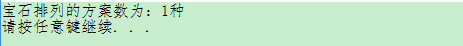
\includegraphics[width=1.0\textwidth]{../img/5.1.PNG}
      \caption{排列宝石问题样例测试}\label{排列宝石问题样例测试}
    \end{figure}
    
   


\end{document} 